\documentclass[../../main.tex]{subfiles}

\begin{document}

\begin{figure}[ht]
\centering
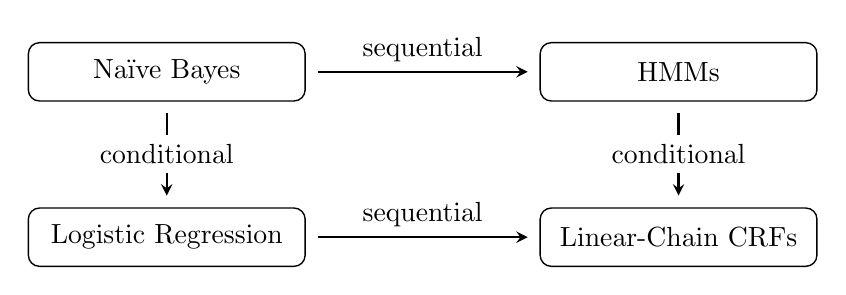
\begin{tikzpicture} [-> , >= stealth,shorten <=0.15cm, shorten >=0.15cm, line width = 0.5pt, minimum width={width("Linear-Chain CRFs")+0.5cm}, minimum height={height("Logistic Regression")+0.5cm}]

\node at (0,0) [draw, rounded corners] (nb) {Na{\"i}ve Bayes};
\node at (0,-2.1) [draw, rounded corners] (logreg) {Logistic Regression};
\node at (6.5,0) (hmm) [draw, rounded corners] {HMMs};
\node at (6.5,-2.1) [draw, rounded corners] (lcrf) {Linear-Chain CRFs};

\path (nb) edge [thick] node [minimum width=0, minimum height=0, fill=white, above=-0.25cm] {conditional}  (logreg);
\path (hmm) edge [thick] node [minimum width=0, minimum height=0, fill=white, above=-0.25cm] {conditional} (lcrf);

\path (nb) edge [thick] node [minimum width=0, minimum height=0, above] {sequential} (hmm);
\path (logreg) edge [thick] node [minimum width=0, minimum height=0, above] {sequential} (lcrf);

\end{tikzpicture}
\caption{Diagram of the relationship between the na{\"i}ve Bayes, logistic regression, HMMs and linear-chain CRFs. Adapted from Figure 2.4 of \autocite{sutton-2012-crfintro}}
\end{figure}

\end{document}